\documentclass[11pt, oneside]{article}
\usepackage[letterpaper, margin=2cm]{geometry}
\usepackage{MATH565}

\begin{document}
\noindent \textbf{\Large{Caleb Logemann \\
MATH 565 Continuous Optimization \\
Final Exam
}}

%\lstinputlisting[language=Python]{H01_23.m}
\begin{enumerate}
    \item % #1
      
    \item % #2
    \item % #3
    \item % #4 Done
      \begin{enumerate}
        \item[(a)] % Done
          This problem can be written as a linear programming problem in the
          following way.
          \begin{align*}
            \max*{} 3P + 4Q - \theta R & \\
            2P + 2Q - R &= 0 \\
            2P + Q &\le 10
            P &\le 8 \\
            P, Q, R &\ge 0
          \end{align*}
          The objective function describes the sale price of the products less
          the cost of the materials.
          The first constraint enforces the amount of materials required for
          the products.
          The second constraint enforces the labor restriction.
          The third constraint enforces the equipment restriction, and the 
          final constraints enforce nonnegativity.
          In standard form, linear programs can be written as
          \begin{align*}
            \max*{} \v{c}^T \v{x} & \\
            \M{A} \v{x} &= b \\
            \v{x} &\ge 0
          \end{align*}
          In order to put our linear program in this form I will introduce
          slack variables, $s_1$ and $s_2$.
          In this case the linear program can be expressed as
          \begin{align*}
            \max*{} \v{c}^T \v{x} & \\
            \M{A} \v{x} &= b \\
            \v{x} &\ge 0
          \end{align*}
          where
          \begin{align*}
            \v{x} =
            \begin{bmatrix}
              P \\
              Q \\
              R \\
              s_1 \\
              s_2
            \end{bmatrix} \qquad
            \v{c} =
            \begin{bmatrix}
              3 \\
              4 \\
              -\theta \\
              0 \\
              0
            \end{bmatrix} \qquad
            \M{A} =
            \begin{bmatrix}
              2 & 2 & -1 & 0 & 0 \\
              2 & 1 & 0 & 1 & 0 \\
              1 & 0 & 0 & 0 & 1
            \end{bmatrix} \qquad
            \v{b} =
            \begin{bmatrix}
              0 \\
              8 \\
              10
            \end{bmatrix}
          \end{align*}

        \item[(b)]
          This linear program is simple enough to be solved graphically.
          The following image shows the feasible region for $P$ and $Q$.
          \begin{center}
            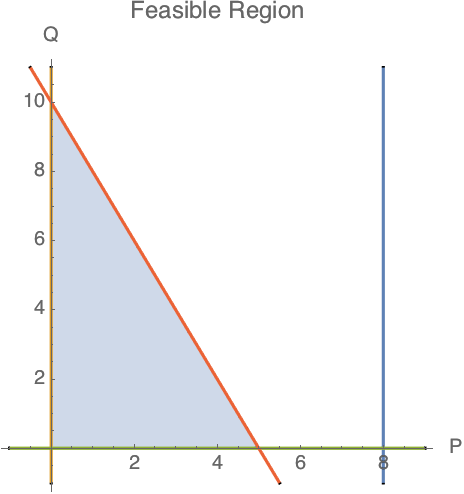
\includegraphics[scale=.7]{Figures/final_1}
          \end{center}
          Note that this problem can be expressed in two dimensions as $R$
          solely depends on $P$ and $Q$ and doesn't have any restrictions.
          Once $P$ and $Q$ are determined $R$ can be determined and the value of
          the objective function can be found.
          Since the objective function is linear, the optimal solution solution
          to this problem must lie on one of the corner points of the feasible
          region or there will be infinitely many optimal solutions along the
          border.
          Therefore I will first consider the 3 corner points of the feasible
          region.
          The first corner point $(0, 0)$ clearly has zero profit, as $P = 0$
          and $Q = 0$ so therefore $R = 0$ and $\v{c}^T \v{x} = 0$.
          At the second corner point $P = 5$ and $Q = 0$, so $R = 10$.
          In this case the profit will be $15 - 10\theta$.
          At the last corner point $Q = 10$ and $P = 0$, thus $R = 20$.
          In this case the profit will be $40 - 20\theta$.
          These two profits are linear with respect to $\theta$ and they are
          not parallel, so therefore there must be values of $\theta$ such that
          $40 - 20\theta > 15 - 10\theta$.
          This can be solved to give an interval on which the profit at $(0, 10)$
          is greater.
          \begin{align*}
            40 - 20\theta &> 15 - 10\theta \\
            35 &> 10\theta \\
            3.5 &> \theta \\
          \end{align*}
          When $\theta < 3.5$, then the profit at $Q = 10$ and $P = 0$ is greater.
          However note that for $\theta > 2$ the profit at $Q = 10$ and $P = 0$
          is negative as $40 - 20\theta = 0$ at $\theta = 2$.
          In this case when $\theta > 2$, then the optimal profit is at $P = 0$
          and $Q = 0$.
          This represents when the raw materials cost more than the value of the
          finished product.
          In this case it is best not to make any of the final product.
          So for $\theta < 2$ the optimal solution is $P = 0$, $Q = 10$, and
          $R = 20$.
          For $\theta > 2$ the optimal solution is $P = 0$, $Q = 0$, and
          $R = 0$.
      \end{enumerate}
\end{enumerate}
\end{document}
